% !TEX root = /media/ueslei/Ueslei/INPE/PCI/Guia_COAWST/main.tex
\chapterimage{ocean2.jpg} % Chapter heading image
\chapter{Introdução}

\bigskip
%%%%%%%%%%%%%%%%%% ROMS %%%%%%%%%%%%%%%%%%%%

\section{Regional Ocean Modeling System}\index{Regional Ocean Modeling System}
\bigskip
\noindent O Regional Ocean Modeling System (ROMS; \cite{Shchepetkin2005}) é um modelo oceânico tridimensional de superfície livre, 
          coordenada vertical sigma (que segue o terreno) e que resolve equações primitivas. Este modelo utiliza a média de Reynolds 
          e o método de diferenças finitas para resolver as equações de Navier-Stokes assumindo aproximações hidrostáticas 
          e de Boussinesq (\cite{Haidvogel2008}).
\bigskip

\noindent As equações hidrostáticas de \textit{momentum} utilizam um esquema de passo de tempo \textit{split-explicit}, 
          onde os modos barotrópico e baroclínico são resolvidos separadamente em distintos números finitos de passos
          de tempo para resolver as equações de superfície livre e momentum integrado na vertical. A estrutura de passos
          de tempo separados mantém a conservação de volume e a preservação de consistência que são necessárias para as equações 
          de traçadores (\cite{Shchepetkin2005,Haidvogel2008}).
\bigskip

\noindent A partir da grade, o modelo resolve as equações na horizontal através de coordenadas curvilíneas ortogonais do 
          tipo Arakawa-C (\cite{Arakawa1977}). Na vertical, as coordenadas seguem as feições do terreno e permitem ajustar a 
          resolução ao longo da coluna d'água. Para garantir a conservação de momentum, a grade utiliza diferenças finitas de
          segunda ordem (\cite{Haidvogel2008}).
\bigskip

\noindent O ROMS é um modelo que possui códigos livre e seu desenvolvimento conta com a contribuição da comunidade de usuários.
          Atualmente, a versão utilizado no COAWST é gerenciado pelo Dr. Hernan Arango da Rutgers University. Para acessar ao 
          código do modelo, é necessário fazer o cadastro no site do ROMS 
          (\textcolor{bleu_cite}{\href{https://www.myroms.org/}{\textit{https://www.myroms.org/}}}) para ter acesso ao código 
          fonte do modelo. É necessário apresentar uma justificativa para se cadastrar no site. O site também conta com um fórum 
          extremamente útil e bastante ativo (\textcolor{bleu_cite}{\href{https://www.myroms.org/forum}{\textit{https://www.myroms.org/forum}}}) 
          perguntas e sugestões sobre problemas na utilização deste modelo.
\bigskip

\noindent Recomenda-se a leitura do Manual Técnico do ROMS, escrito por \textcite{hedstrom2018}. Este manual conta com diversas 
          informações sobre as equações e algorítmos do modelo e exemplos de casos-teste. 


%%%%%%%%%%%%%%%%%%%% Sea Ice %%%%%%%%%%%%%%%%%%%%

\section{Budgell's Sea Ice Model}\index{Budgell's Sea Ice Model}
\bigskip

\noindent O Modelo de Gelo Marinho, proposto por \textcite{Budgell2005}, possui os mesmos passos de tempo e grade do ROMS e 
          compartilha a mesma estrutura de codificação paralela para uso com Message Passing Import (MPI). Dessa maneira, 
          permite a modelagem dinâmica e termodinâmica onde houver o predomínio de gelo marinho, como por exemplo em altas latitudes. 
\bigskip

\noindent Os principais atributos do modelo, de acordo com \textcite{hedstrom2018}, são:
\bigskip
\begin{itemize}
    \item Dinâmica elástica-viscosa de \textcite{Hunke1997} e \textcite{Hunke2001};
    \item Termodinâmica proposta por \textcite{Mellor1989};
    \item Coordenadas curvilíneas-ortogonais;
    \item Grade Arakawa-C proposto  por \textcite{Arakawa1977};
    \item Advecção de traçadores proposta por \textcite{Smolarkiewicz1990};
    \item Parametrização de gelo proposta por \textcite{Lemieux2015}.
\end{itemize}
\bigskip


%%%%%%%%%%%%%%%%%%%% WRF %%%%%%%%%%%%%%%%%%%%

\section{Weather Research \& Forecasting Model}\index{Weather Research \& Forecasting Model}
\bigskip

\noindent O Weather Research and Forecasting (WRF; \cite{Skamarock2008}) é um modelo desenvolvido pelo National Centers for 
          Environmental Prediction (NCEP), National Center for Atmospheric Research (NCAR) e grupos de pesquisa de diferentes
          universidades.
\bigskip

\noindent Para integrar no tempo as equações governantes, o Advanced Research WRF (ARW) utiliza modos de baixa freqüência que são integrados 
          utilizando o esquema de Runge-Kutta de terceira ordem, e os modos acústicos e de ondas de gravidade (alta frequência) integrados 
          com passo de tempo menor. Dessa maneira, se mantém a estabilidade numérica, através de um esquema “forward-backward” para 
          os modos acústicos que se propagam horizontalmente, e de um esquema implícito para modos acústicos de propagação 
          vertical e oscilações de empuxo (\cite{Skamarock2008}).
\bigskip

\noindent O modelo WRF utiliza uma grade do tipo Arakawa-C (\cite{Arakawa1977}), onde as velocidades normais estão
          escalonadas a meio comprimento da grade das variáveis termodinâmicas, conforme via representação esquemática ilustrada
          na Figura \textcolor{bleu_cite}{\ref{gradeswrf}}.
\bigskip

\begin{figure}[H]
    \centering
    \captionsetup{justification=centering}
    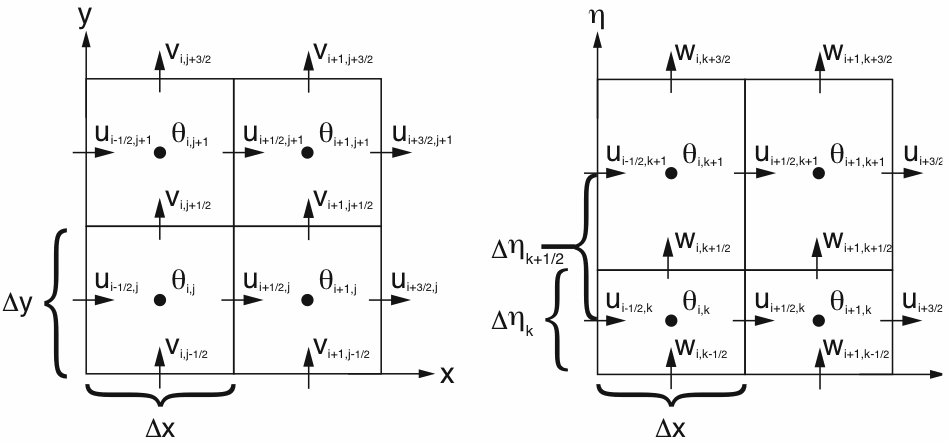
\includegraphics[width=0.80\textwidth]{grid_new.png}
    \caption{Grade horizontal e vertical do Weather Research and Forecast (WRF) em Arawaka-C. As componentes horizontal e vertical
                        da velocidade (\textbf{u}, \textbf{v} e \textbf{w}) estão posicionados ao longo das faces das grades e as variáveis termodinâmicas
                        (\straighttheta) estão posicionados no centro de cada grade. \newline Fonte: \textcite{Skamarock2008}.}
    \label{gradeswrf}
\end{figure}
\bigskip

\noindent É importante ressaltar que o WRF, sem o acoplamento com outros modelos, simula a rugosidade da superfície 
          baseada na Relação de rugosidade com o cisalhamento do vento proposta por \textcite{Charnock1955},
          como exemplificado na Equação \textcolor{bleu_cite}{\ref{equacao1}}:
\bigskip

\begin{equation}
Z_{0} = Z_{ch} \frac{u_{*}^{2}}{g}
\label{equacao1}
\end{equation}

\bigskip

\noindent Onde \textit{Z\textsubscript{0}} é a rugosidade, \textit{Z\textsubscript{ch}} é o parâmetro de Charnock 
         (um valor adimensional de 0,018), \textit{u\textsubscript{*}} a velocidade de fricção (m/s) e \textit{g} a 
         aceleração da gravidade (9,81 m/s\textsuperscript{2}).
\bigskip

\noindent Para baixar o WRF, acesse: \textcolor{bleu_cite}{\href{http://www2.mmm.ucar.edu/wrf/users/download/get\_source.html}{\textit{http://www2.mmm.ucar.edu/wrf/users/download/get\_source.html}}}
\bigskip

%%%%%%%%%%%%%%%%%%% SWAN %%%%%%%%%%%%%%%%

\section{Simulating Waves Nearshore}\index{Simulating Waves Nearshore}
\bigskip

\noindent O Simulating Waves Nearshore (SWAN; \cite{Booij1999,Booij1996}) é um modelo de terceira geração, 
          concebido para computar em regiões costeiras com águas rasas e correntes locais. O modelo é amplamente utilizado na previsão numérica do 
          espectro de ondas em regiões costeiras, estuários, canais e outros, podendo utilizar campos de vento, batimetria e 
          correntes fornecidos por outros modelos \parencite{Booij1999,Booij1996}.
\bigskip

\noindent \textcite{Dasilva2013} e \textcite{Booij1999,Booij1996} elencam as principais características do SWAN:
\bigskip

\begin{itemize}
\item refração de onda com profundidade variável;
\item empinamento induzido pela profundidade e corrente;
\item geração e propagação de ondas pelo vento;
\item dissipação por \textit{whitecapping};
\item dissipação pela quebra de ondas induzida pela profundidade;
\item dissipação devido à fricção com o fundo;
\item interações não lineares tipo onda-onda triplas e quádruplas;
\item difração.
\end{itemize}
\bigskip

%%%%%%%%%%%%%%%%%%% MCT %%%%%%%%%%%%%%%%
\section{Model Coupling Toolkit}\index{Model Coupling Toolkit}
\bigskip

\noindent O Model Coupling Toolkip (MCT; \cite{Larson2005,Jacob2005,Warner2008}) é um conjunto de rotinas livres, 
          escritas em Fortran 90 que permitem a transmissão e transformação dos diferentes dados necessários ao acoplamento
          de modelos. Durante a inicialiação, os domínios dos modelos são decompostos em segmentos que são distribuídos
          entre os processadores, permitindo que os modelos sejam acoplados também de forma paralela.
\bigskip

\noindent Segundo o site do MCT ((\textcolor{bleu_cite}{\href{http://www.mcs.anl.gov/research/projects/mct/}{\textit{http://www.mcs.anl.gov/research/projects/mct/}}}), 
          ele fornece os seguintes serviços de acoplamento de núcleo:
\bigskip

\begin{itemize}
\item um registro das componentes dos modelos;
\item descritores de decomposição do domínio;
\item ferramentas paralelizadas para interpolação \textit{intergrid};
\item ferramentas para mesclar dados de entre vários componentes;
\item um modelo de programação semelhante ao MPI (Message Passing Interface).
\end{itemize}
\bigskip

%%%%%%%%%%%%%%%%%%%%% SCRIP %%%%%%%%%%%%%%
\section{Spherical Coordinate Remapping Interpolation Package}\label{scripsecao}
\bigskip

\noindent O  Spherical Coordinate Remapping Interpolation Package (SCRIP; \cite{Jones1999,Jones1998}) 
          está disponível gratuitamente em \textcolor{bleu_cite}{\href{http://oceans11.lanl.gov/trac/SCRIP}{\textit{http://oceans11.lanl.gov/trac/SCRIP}}} 
          e é distribuído junto com o COAWST. Este pacote é usado para projetos que utilizam mais de um modelo e que possuem grades 
          horizontais diferentes, ou seja com diferentes resoluções espaciais. O SCRIP gerará os pesos de interpolação que serão 
          usados para remapear os dados entre as distintas grades dos diferentes modelos.
\bigskip

\noindent No COAWST, o SCRIP foi modificado para gerar um único arquivo (no formato NetCDF) que contém o resultado do cálculo 
          dos pesos baseado nas grades dos modelos.

\bigskip
%%%%%%%%%%%%%%%%%%% COAWST %%%%%%%%%%%%%%%%

\section{Coupled-Ocean-Atmosphere-Wave-Sediment Transport Modeling System}\index{Coupled-Ocean-Atmosphere-Wave-Sediment Transport Modeling System}
\bigskip
\noindent O Coupled Ocean-Atmosphere-Wave-Sediment Transport Modeling System (COAWST; \cite{Warner2010,Warner2008}), 
          é composto pelo modelo atmsoférico WRF, o modelo oceânico ROMS, o modelo de ondas SWAN e o modelo de transporte de sedimentos
          da Community Sediment Transport Modeling Project (CSTM; \cite{Warner2008}), acoplados pelo MCT (\cite{Warner2010,Warner2008}). 
          A frequência com que estas informações são trocadas entre os diferentes modelos é ajustada pelo usuário.
\bigskip

\noindent O acoplamento entre os modelos permite que os diferentes processos físicos que ocorrem nos meios oceânico e atmosférico, 
          sejam identificados e analisados com maior acurácia em comparação com simulações sem acoplamento ativo. (\cite{Pullen2018, Miller2018}).
\bigskip

\begin{tcolorbox}[enhanced,
  grow to left by   = 0cm,
  grow to right by  = 0cm,
  enlarge top by    = 0cm,
  enlarge bottom by = 0cm,
  tcbox raise base,
  boxrule           = 1.0pt,
  left              = 18mm,
  colframe          = red!50!black,coltext=red!25!black,colback=red!10!white,
  overlay           = {\begin{tcbclipinterior}\fill[red!75!blue!50!white] (frame.south west)
    rectangle node[text=white,font=\sffamily\bfseries\footnotesize,rotate=0] {ATENÇÃO} ([xshift=18mm]frame.north west);\end{tcbclipinterior}}]
Este guia não usa o CSTM. Caso esteja interessado, há um estudo sobre a transferência de sedimentos durante o furacão Isabel (2003) realizado por \textcite{Warner2010}.
\end{tcolorbox}
\bigskip


\noindent Conforme a Figura \textcolor{bleu_cite}{\ref{acopla}}, as informações trocadas entre modelos são:
\bigskip

\begin{itemize}
\item WRF -> ROMS: cisalhamento de superfície e fluxo de calor líquido (calculado no ROMS a partir das componentes dos fluxos de calor latente e sensível e radiação de ondas curta e longa, a pressão atmosférica, umidade relativa, temperatura do ar, nuvens, precipitação e as componentes do vento;
\item ROMS -> WRF: temperatura da superfície do mar;
\item SWAN -> ROMS: direção da onda em superfície e no fundo, altura, comprimento, período, dissipação de energia e velocidade orbital inferior;
\item ROMS -> SWAN: batimetria, elevação da superfície, altura da superfície do mar e correntes médias em profundidade;
\item SWAN -> WRF: rugosidade da superfície do mar (calculado no WRF a partir da altura significativa da onda, comprimento e período);
\item WRF -> SWAN: vento a 10m de altura.
\end{itemize}
\bigskip

\begin{figure}[H]
    \begin{tikzpicture}[->,
        >=stealth',
        shorten >=1pt,
        auto,
        node distance=2.75cm, 
        state/.style={
        draw=black,
        fill=bleu_cite,
        circle, 
        text=black,
        text width={width("ROMS")},
        minimum size=1.5cm,
        align=center,
        rounded corners,
        font=\small}]

        \hspace{5cm}
        \node[state] (A)  {\small WRF};
        \node[state] (C)  [right=4cm of A] {\small ROMS \scriptsize{Sea ice}};
        \node[state] (B)  [below=4cm of C,right of= A] {\small SWAN};

        \path (A) edge [draw=black, bend right=20] node[sloped, align=center, below,font=\tiny]  {U\textsubscript{wind}, V\textsubscript{wind}, P\textsubscript{atm}, RH, \\T\textsubscript{air}, Cloud, Rain, \\SW\textsubscript{rad}, LW\textsubscript{rad}} (C); % WRF->ROMS
        \path (C) edge [draw=black, bend right=20] node[sloped, align=center, below,font=\tiny] {SST} (A);
        \path (A) edge [draw=black, bend right=20] node[sloped, align=center, below,font=\tiny] {U\textsubscript{wind}, \textsubscript{wind}} (B); 
        \path (B) edge [draw=black, bend right=20] node[sloped, align=center, below,font=\tiny] {L\textsubscript{wave}, H\textsubscript{wave}} (A);
        \path (B) edge [draw=black, bend right=20] node[sloped, align=center, below,font=\tiny] {L\textsubscript{wave}, H\textsubscript{wave}, D\textsubscript{wave}, \\T\textsubscript{surface}, T\textsubscript{bottom}, Q\textsubscript{B}, \\W\textsubscript{dissipation}, U\textsubscript{b}} (C); 
        \path (C) edge [draw=black, bend right=20] node[sloped, align=center, below,font=\tiny] {U\textsubscript{s}, V\textsubscript{s}, Bathymetry, \\Bottom Elevation} (B); 
        \node[align=center,font=\bfseries, yshift=2em] (title) at (current bounding box.north) {\small Coupled Ocean-Atmosphere-Wave-\\\small Sediment Transport modeling system \\\small v3.4};
    \end{tikzpicture}
\captionsetup{justification=centering}
\caption{Esquema sobre a troca de informações entre três modelos que compõe o sistema COAWST. (\cite{Warner2008})}
\label{acopla}
\end{figure}
\bigskip

\noindent A página do Woods Hole Coastal and Marine Science Center fornece, em caráter experimental, uma apresentação em 
          tempo real da integração do COAWST (Temperatura da Superfície do Mar, Altura da Superfície do Mar, Altura Significativa
          de Ondas, Vetores de Corrente e Vento e dispersão de Sedimentos) para o leste dos Estados Unidos e Golfo do México.
          O conteúdo está disponível em \textcolor{bleu_cite}{\href{https://woodshole.er.usgs.gov/project-pages/cccp/public/COAWST.htm}{\textit{https://woodshole.er.usgs.gov/project-pages/cccp/public/COAWST.htm}}}.
\bigskip

%%%%%%%%%%%%%%%%%%%%%  PYTHON %%%%%%%%%%%%%%%%%%%%%%%%%%%
\section{Python}\index{Python}
\bigskip

\noindent O Python é uma linguagem de programação projetada com a filosofia de enfatizar a importância 
          do esforço do programador sobre o esforço computacional. Prioriza a legibilidade do código sobre 
          a velocidade ou expressividade.
\bigskip

\noindent A linguagem preza pela simplicidade e eficácia e possui uma ampla e ativa comunidade, o que facilita muito ao
         usuário em caso de dúvidas, pois há na internet um extenso acervo de bibliotecas e documentação.
\bigskip

\noindent O Python Brasil (\textcolor{bleu_cite}{\href{http://python.org.br}{\textit{http://python.org.br}}}) oferece
          grande auxílio para iniciantes na linguagem, disponibilizando introduções ((\textcolor{bleu_cite}{\href{http://python.org.br/introducao}{\textit{http://python.org.br/introducao}}}) 
          e também um guia ((\textcolor{bleu_cite}{\href{http://python.org.br/cientifico}{\textit{http://python.org.br/cientifico}}}) para o uso do 
          Python no meio científico.



%%%%%%%%%%%%%%%%%%%%%%%%%%% MATERIAIS %%%%%%%%%%%%%%%%%%%%%%%%%%%%%
\section{Materiais necessários para o uso deste guia}\index{Materiais}
\bigskip

\noindent Este guia utiliza um cluster com capacidade de paralelização de operações como exemplo para compilar. Para compilar o COAWST \textcolor{red}{v3.4}
          em um computador sem comunicação paralela, utilize o manual original, disponível no repositório original do modelo. 
          Veja como baixar o COAWST na seção \textcolor{bleu_cite}{\ref{coawstbaixa}}.
\bigskip

\noindent Para gerar as condições e a grade do modelo oceânico ROMS, utilizamos o Ubuntu 18.04 LTS. Isso é importante pois sistemas
          operacionais diferentes podem gerar conflitos ao utilizar o pacote \textit{model2roms}. que gera as os arquivos necessários para utilizar o ROMS.